\documentclass[usenames,dvipsnames,8pt,aspectratio=169]{beamer}
\usepackage{amsmath,amsfonts,amssymb}
\usepackage{mathtools}
\usepackage{etex} %for Windows
\usepackage[utf8]{inputenc}
\usepackage[english, russian]{babel} 
%\usepackage{microtype}			% Better interword spacing and additional kerning.
\usepackage{ellipsis}			% Adjusted space with \dots between two words.
\usepackage{graphicx}
\usepackage{pstricks}

\usepackage{xcolor}


\usepackage{changepage}

\usepackage{algorithm}
\usepackage{algpseudocode}
%\usepackage[]{algorithm2e}
%\usepackage{algorithmic}

%\usepackage{tcolorbox}


\usepackage{caption}
\usepackage{subcaption}
%\usepackage{stackengine}


\usepackage{tikz}
\usetikzlibrary{tikzmark,calc}
\usetikzlibrary{positioning, backgrounds}
\usetikzlibrary{arrows, chains, matrix, scopes, patterns, shapes, fit}
\usetikzlibrary{mindmap,trees,shadows}
\usetikzlibrary{decorations.pathreplacing}
%\usetikzlibrary{crypto.symbols}

\usepackage{pgfplots}

\pgfmathdeclarefunction{gauss}{2}{%
	\pgfmathparse{1/(#2*sqrt(2*pi))*exp(-((x-#1)^2)/(2*#2^2))}%
}


\tikzset{
	invisible/.style={opacity=0},
	visible on/.style={alt={#1{}{invisible}}},
	alt/.code args={<#1>#2#3}{%
		\alt<#1>{\pgfkeysalso{#2}}{\pgfkeysalso{#3}} % \pgfkeysalso doesn't change the path
	},
}

\newcommand\strikeout[2][]{%
	\begin{tabular}[b]{@{}c@{}} 
		\makebox(0,0)[cb]{{#1}} \\[-0.2\normalbaselineskip]
		\rlap{\color{Orange}\rule[0.5ex]{\widthof{#2}}{1.5pt}}#2
\end{tabular}}

\newcommand\Fontvi{\fontsize{11}{13.2}\selectfont}

\usepackage{listings} % for C++ code

\usepackage{braket}
%\usepackage[braket, qm]{qcircuit}



\usepackage[T1]{fontenc}
%\usepackage[sfdefault,scaled=.85]{FiraSans}
%\usepackage{newtxsf}
%\usepackage[nomap]{FiraMono}





\usefonttheme[onlymath]{serif}
\renewcommand\sfdefault{cmbr}

\renewcommand{\bfdefault}{sb}

\definecolor{CharCoalDark}{RGB}{13, 16, 19}
\definecolor{Orange}{RGB}{255, 165,0}
\definecolor{DarkOrange}{RGB}{255, 165,0}
\definecolor{LightSalmon}{RGB}{255, 160, 122}
\definecolor{LeafGreen}{RGB}{34, 139,  34}
\definecolor{Coral}{RGB}{255, 127, 80}
\definecolor{DarkTurquoise}{RGB}{0, 206, 209}

%\newtheorem{defRus}{Определение}
%\newtheorem{thmRus}{Теорема}
%s\newtheorem{corRus}{Следствие}


\setbeamercolor{background canvas}{bg=CharCoalDark}

\setbeamerfont{title}{series=\bfseries}
\setbeamercolor{title}{fg=Orange}
\setbeamercolor{section in toc}{fg=white}
\setbeamercolor{frametitle}{fg=Orange}
\setbeamercolor{normal text}{fg=white}
%\setbeamercolor{normal text}{fontsize=12pt}
\setbeamercolor{itemize item}{fg=Orange}
\setbeamercolor{enumerate item}{fg=Orange}
\setbeamercolor{enumerate item item}{fg=Orange}
\setbeamercolor{itemize item item}{fg=Orange}
\setbeamercolor{enumerate item}{fg=Orange}
\setbeamercolor{block title}{bg=DarkOrange,fg=white}
\setbeamerfont{block title}{series=\bfseries}

\setbeamertemplate{itemize item}[circle]
\setbeamertemplate{eumerate subitem}{\color{Orange}[$\checkmark$]}
\setbeamertemplate{itemize subitem}{\color{Orange}\Large$\textbullet$}
\setbeamertemplate{itemize subitem}{\color{Orange} \tiny $\blacksquare$}

% footnote without a marker
\newcommand\blfootnote[1]{%
	\begingroup
	\renewcommand\footnoterule{}
	\renewcommand\thefootnote{}\footnote{#1}%
	\addtocounter{footnote}{-1}%
	\endgroup
}

\newcommand*{\Scale}[2][4]{\scalebox{#1}{\ensuremath{#2}}}%

\newcommand\Item[1][]{%
	\ifx\relax#1\relax  \item \else \item[#1] \fi
	\abovedisplayskip=0pt\abovedisplayshortskip=0pt~\vspace*{-\baselineskip}}

\pgfdeclareradialshading{ring}{\pgfpoint{0cm}{0cm}}%
{rgb(0cm)=(1,1,1);
	rgb(0.7cm)=(1,1,1);
	rgb(0.719cm)=(1,1,1);
	rgb(0.72cm)=(0.975,0,0);
	rgb(0.9cm)=(1,1,1)}

\usepackage[absolute,overlay]{textpos} %to clip to a corner
\newcommand\FrameText[1]{%
	\begin{textblock*}{\paperwidth}(\textwidth-35pt, 10 pt)
		\raggedright #1\hspace{.5em}
\end{textblock*}}

\makeatletter
\let\save@measuring@true\measuring@true
\def\measuring@true{%
	\save@measuring@true
	\def\beamer@sortzero##1{\beamer@ifnextcharospec{\beamer@sortzeroread{##1}}{}}%
	\def\beamer@sortzeroread##1<##2>{}%
	\def\beamer@finalnospec{}%
}
\makeatother

\AtBeginSection[]
{
	\begin{frame}<beamer>
		\frametitle{Outline}
		\tableofcontents[currentsection]
	\end{frame}
}



\newcommand{\AxisRotator}[1][rotate=0]{%
	\tikz [x=0.4cm,y=1.0cm,line width=.2ex,-stealth,#1] \draw[color=Orange] (0,0) arc (-150:150:2 and 1);%
}

\title{Лекция №5 \\[10pt]
	Часть 1. Схема криптографической подписи}

\date{ Елена Киршанова \\  \textbf{Курс ``Основы криптографии''} \\  }



\setbeamertemplate{navigation symbols}{} %removes navigation

% proper highlightling of a code-snippet
\lstset{language=C++,
	keywordstyle=\color{magenta},
	stringstyle=\color{Goldenrod},
	commentstyle=\color{gray},
	breaklines=false,
	%morecomment=[l][\color{magenta}]{\#}
}

%\setlength{\parskip}{8pt}
% ==================================================================
% Definitions for this paper
% ==================================================================
\mathchardef\hyphen="2D

\usepackage{multirow}
\usepackage{multicol} % For multiple coloumn environments
%\usepackage{stmaryrd} % For set brackets
% \setlength{\columnsep}{15pt} % Defining the coloumn seperation
% \setlength{\columnseprule}{1pt} % Place a line between coloumns
% \newcommand{\tab}{\hspace*{2em}}

%subscripts

\newcommand*\SmallTextScript[2]{{\mathchoice{\displaystyle #2}
		{\textstyle #2}%dito
		{\scalebox{#1}{\ensuremath{\scriptstyle #2}}}%
		{\scalebox{#1}{\ensuremath{\scriptscriptstyle #2}}}%
}}


% ADVERSARIES AND SUCH
\newcommand*{\poly}{\ensuremath{\mathrm{poly}}}
\newcommand*{\eps}{\ensuremath{\varepsilon}}
\newcommand*{\alg}{\ensuremath{\mathcal{A}}}

% GROUPS/DISTRIBUTIONS/SETS/LISTS
\newcommand{\N}{{{\mathbb N}}}
\newcommand{\Z}{{{\mathbb Z}}}
\newcommand*{\IZ}{\ensuremath{\mathbb{Z}}}
\newcommand*{\IN}{\ensuremath{\mathbb{N}}}
\newcommand*{\IQ}{\ensuremath{\mathbb{Q}}}
\newcommand{\R}{{{\mathbb R}}}
\newcommand*{\IR}{{{\mathbb R}}}
\newcommand{\Zp}{\ints_p} % Integers modulo p
\newcommand{\Zq}{\ints_q} % Integers modulo q
\newcommand{\Zn}{\ints_N} % Integers modulo N
\newcommand{\F}{\ensuremath{\mathbb{F}}}
\newcommand{\CC}{\ensuremath{\mathbb{C}}}

\newcommand{\GF}{\ensuremath{\mathbb{F}_2}}
\newcommand{\GFn}{\ensuremath{\mathbb{F}^n_2}}

%%% ALGORITHMS/PROCEDURES %%%
\newcommand{\Dec}{\textsf{Dec}}
\newcommand{\Enc}{\textsf{Enc}}
\newcommand{\KeyGen}{\textsf{KeyGen}}
\newcommand{\Gen}{\textsf{Gen}}
\newcommand{\sk}{\textsf{sk}}
\newcommand{\pk}{\textsf{pk}}
\newcommand{\vk}{\textsf{vk}}
\newcommand{\mesS}{\ensuremath{\mathcal{M}}}
\newcommand{\keyS}{\ensuremath{\mathcal{K}}}
\newcommand{\cipS}{\ensuremath{\mathcal{C}}}
\newcommand{\tagS}{\ensuremath{\mathcal{T}}}
\newcommand{\mactag}{\textsf{tag}}
\newcommand{\Hash}{\ensuremath{\mathcal{H}}}
\newcommand{\EID}{\ensuremath{\mathtt{EphID}}}


\newcommand{\adv}{\ensuremath{\mathcal{A}}}

\newcommand{\LWE}{\mathsf{LWE}}
\newcommand{\DCP}{\mathsf{DCP}}
\newcommand{\EDCP}{\mathsf{EDCP}}
\newcommand{\UEDCP}{\mathsf{U \text{-} EDCP}}
\newcommand{\GEDCP}{\mathsf{G \text{-} EDCP}}



%% Landau and proba
\newcommand{\bigO}{\mathcal{O}}
\newcommand*{\OLandau}{\bigO}
\newcommand*{\WLandau}{\Omega}
\newcommand*{\xOLandau}{\widetilde{\OLandau}}
\newcommand*{\xWLandau}{\widetilde{\WLandau}}
\newcommand*{\TLandau}{\Theta}
\newcommand*{\xTLandau}{\widetilde{\TLandau}}
\newcommand{\smallo}{o} %technically, an omicron
\newcommand{\wLandau}{\omega}
\newcommand{\negl}{\mathrm{negl}}
\newcommand*\PROB\Pr 
\DeclareMathOperator*{\EXPECT}{\mathbb{E}}
\DeclareMathOperator*{\VARIANCE}{\mathbb{V}}
\DeclareMathOperator*{\LOGBIAS}{\mathbb{LB}}

\newcommand{\supp}{\ensuremath{\mathsf{sup}}}
\newcommand{\Distr}{\ensuremath{\mathcal{D}}}

% Lattices

% \newcommand{\coset}{\Lambda} % Lambda Lattice
% \newcommand{\cosetPerp}{\Lambda^{\bot}} % Lambda_Perp Lattice
% \newcommand{\gadget}{\textbf{G}} %Gaget matrix
% \newcommand{\mes}{\textbf{m}} %message vector
% \newcommand{\AMat}{\textbf{A}} %A matrices
% \newcommand{\BMat}{\textbf{B}} %B matrices
% \newcommand{\RMat}{\textbf{R}} %R matrices
% \newcommand{\HMat}{\textbf{H}} %H matrices
% \newcommand{\XMat}{\textbf{X}} %H matrices
% \newcommand{\mbar}{\bar{m}} %mBar dimension
% % \newcommand{\gauss}{\mathcal{D}} % gaussian distribution
% \newcommand{\Id}{\textbf{I}} % Identity matrix
% \newcommand{\er}{\textbf{e}} % gaussian distr. vectors
% % \newcommand{\cipher}{\textit{c}} % ciphertext
% \newcommand{\Olwe}{\mathcal{O}_{\textsf{LWE}}} %LWE oracle
% \newcommand{\OSample}{\mathcal{O}_{Sample}} %LWE oracle
% \newcommand{\SigmaB}{\boldsymbol{\Sigma}} %semi-deifinite matrix Sigma%
% % \newcommand{\mods}{\text{ mod}}


%Vectors and Matrices

\newcommand{\AMat}{\mathbf{A}} %A matrices
\newcommand{\BMat}{\mathbf{B}} %B matrices
\newcommand{\DMat}{\mathbf{D}} %Diagonal


\newcommand{\HMat}{\ensuremath{\mathbf{H}}}
\newcommand{\QMat}{\ensuremath{\mathbf{Q}}}
\newcommand{\Id}{\ensuremath{\mathbf{I}}}
\newcommand{\ZeroM}{\textbf{0}} % Zero matrix

\newcommand{\avec}{\ensuremath{\mathbf{a}}}
\newcommand{\bvec}{\ensuremath{\mathbf{b}}}
\newcommand{\cvec}{\ensuremath{\mathbf{c}}}
\newcommand{\evec}{\ensuremath{\mathbf{e}}}
\newcommand{\rvec}{\ensuremath{\mathbf{r}}}
\newcommand{\svec}{\ensuremath{\mathbf{s}}}
\newcommand{\tvec}{\ensuremath{\mathbf{t}}}
\newcommand{\vvec}{\ensuremath{\mathbf{v}}}
\newcommand{\zvec}{\ensuremath{\mathbf{z}}}
\newcommand{\xvec}{\ensuremath{\mathbf{x}}}
\newcommand{\yvec}{\ensuremath{\mathbf{y}}}
\newcommand{\uvec}{\ensuremath{\mathbf{u}}}
\newcommand{\zerovec}{\ensuremath{\mathbf{0}}}

\newcommand{\nth}{^{\mathrm{th}}}
\newcommand{\nd}{^{\mathrm{nd}}}

\newcommand{\RepMMT}{\ensuremath{\mathcal{R}_{\protect\SmallTextScript{0.70}{\texttt{MMT}}}}}
\newcommand{\RepBJMM}{\ensuremath{\mathcal{R}_{\protect\SmallTextScript{0.70}{\texttt{BJMM}}}}}
\newcommand{\XOR}{\ensuremath{\mathtt{3XOR}}}


% % % % % \newcommand{\mb}[1]{\mathbf{#1}} % does not compile otherwise
%%% Removed by Gotti; this is just asking to screw up with packages that (properly) define \mb (mathbold)

% \newcommand{\bL}{\|\bvec_1\|} % b1 length that appears way too often
% \newcommand{\dL}{\|\dvec_1\|} % b1 length that appears way too oftend

%Norms and Scalar products

\newcommand*\abs[1]{\left\lvert#1\right\rvert}
\newcommand*\norm[1]{\left\lVert#1\right\rVert}
\newcommand*\normalabs[1]{\lvert#1\rvert} 
\newcommand*\normalnorm[1]{\lVert#1\rVert}
\newcommand*\bignorm[1]{\bigl\lVert#1\bigr\rVert}
\newcommand*\bigabs[1]{\bigl\lvert#1\bigr\rvert}
\newcommand*\Bigabs[1]{\Bigl\lvert#1\Bigr\rvert}
\newcommand*{\ScProd}[2]{\ensuremath{\langle#1\mathbin{,}#2\rangle}} %Scalar Product
% \newcommand*{\ScProd}[2]{\ensuremath{\langle#1 \:{,}\:#2\rangle}} %Scalar Product
\newcommand*{\bigScProd}[2]{\ensuremath{\bigl\langle#1\mathbin{,}#2\bigr\rangle}} %Scalar Product
\newcommand*{\BigScProd}[2]{\ensuremath{\Bigl\langle#1\mathbin{,}#2\Bigr\rangle}} %Scalar Product
\newcommand{\dist}{\ensuremath{\text{dist}}}


%Some other math operators

\DeclareMathOperator{\Span}{Span} %span of vectors
\DeclareMathOperator{\vol}{\mathrm{vol}} %volume
\DeclareMathOperator{\LW}{LambertW} %Lambert W function
\DeclareMathOperator{\SD}{SD}
\DeclareMathOperator{\gradient}{grad}
\DeclareMathOperator{\TRACE}{Tr}
\newcommand*{\dDR}{\mathrm{d}} %de-Rham-Differential (the d in dx, dy, dz and so on)


%Lists
\renewcommand{\L}{\ensuremath{\mathcal{L}}}

\renewcommand{\P}{\ensuremath{\mathcal{P}}}

\newcommand*{\Lout}{\ensuremath{\L_{\mkern-0.5mu\protect\SmallTextScript{0.85}{\textup{out}}}}}
\newcommand*{\Sout}{\ensuremath{S_{\mkern-0.5mu\protect\SmallTextScript{0.85}{\textup{out}}}}}
\newcommand{\wt}{\ensuremath{\mathit{wt}}}


\newcommand*{\softO}{\widetilde{\bigO}}

\newcommand{\const}{\mathsf{c}} 


\newcommand{\transpose}{\mkern0.7mu^{\mathsf{ t}}}

%proper overline reduced by 1.5mu
\newcommand{\overbar}[1]{\mkern 1.5mu\overline{\mkern-1.5mu#1\mkern-1.5mu}\mkern 1.5mu}

\DeclareMathOperator{\erf}{erf} %error function
\DeclareMathOperator{\erfc}{erfc} %complementary error function
\newcommand{\Er}{\ensuremath{\mathrm{Er}}} %complementary error function


% LATTICES

\newcommand{\Lat}{\ensuremath{\mathcal{L}}}
\newcommand*{\Sphere}[1]{\ensuremath{\mathsf{S}^{#1}}}
%\DeclareMathOperator{\Conf}{Conf}
\newcommand{\Conf}{\mathcal{C}}

%Thick line for table
\setlength{\doublerulesep}{0pt}
\newcommand{\thickline}{\hline\hline\hline}


%circled text
\newcommand*\circled[1]{\tikz[baseline=(char.base)]{
    \node[shape=circle,draw,inner sep=0.3 pt] (char) {\scriptsize #1};}}


%Fix Algorithmicx package
\def\NoNumber#1{{\def\alglinenumber##1{}\State #1}\addtocounter{ALG@line}{-1}}

%For comments
\newcommand{\GColor}{ForestGreen}  %Damiens' color
\newcommand{\EColor}{MidnightBlue} %Elena's color

\newcommand*{\E}[1]{{\color{\EColor} #1} } 
\newcommand*{\G}[1]{{\color{\GColor} #1} } 

%Proper limit with the subscript underneath
% \newcommand{\Lim}[1]{\raisebox{0.5ex}{\scalebox{0.8}{$\displaystyle \lim_{#1}\;$}}}


%TIKZ dense dotted pattern

\pgfdeclarepatternformonly{my dots}{\pgfqpoint{-1pt}{-1pt}}{\pgfqpoint{2.0pt}{2.0pt}}{\pgfqpoint{2pt}{2pt}}%
{
	\pgfpathcircle{\pgfqpoint{0pt}{0pt}}{.35pt}
	\pgfpathcircle{\pgfqpoint{1pt}{1pt}}{.35pt}
	\pgfusepath{fill}
}


\tikzset{
	master/.style={
		execute at end picture={
			\coordinate (lower right) at (current bounding box.south east);
			\coordinate (upper left) at (current bounding box.north west);
		}
	},
	slave/.style={
		execute at end picture={
			\pgfresetboundingbox
			\path  (lower right)rectangle (upper left) ;
		}
	}
} %all defs
\begin{document}
	
\begin{frame}
	\titlepage
\end{frame}

\begin{frame}{Агенда}
	
	\Large
	\begin{itemize}
		\itemsep 10 pt
		\item Зачет в субботу 12/11 в 10:10 в Webinar
		\url{https://events.webinar.ru/58831339/1604249105}
		\item Доп. защита лабраторных в пятницу 11/11 в 10:00 в Webinar
		\url{https://events.webinar.ru/58831339/2144800577}
	\end{itemize}
	
\end{frame}

\begin{frame}{Схема цифровой подписи: зачем нужна?}
	\large 
	\begin{center}
Обмен ключами + Симметрическое шифрование =  {\color{Orange}{конфидециальность} } 
	\end{center}
Но
	\begin{itemize}
		\itemsep 10pt
		\item протокол обмена ключами Диффи-Хэллмана {\color{Orange} подвержен активным атакам} 
		\item  он не обеспечивает {\color{Orange} целостность} передаваемых данных
		\item он не обеспечивает {\color{Orange} аутентификацию}
	\end{itemize}

\vspace{15pt}

Наша цель: обеспечить целостность и аутентификацию, как схема MAC,  но в асимметриченом  {\color{Orange} открытым} мире.\\[10pt]

%\centering

\Large Асимметричная версия МАС'a -- {\color{Orange} криптогрфическая схема подписи}
\end{frame}



\begin{frame}{Схема подписи: определение}
\Large

{\color{Orange}{Схема подписи}} состоит из трех ppt алгоритмов
\begin{itemize}
	\itemsep 10pt
	\item Генерация ключа: $(\sk, \vk) \leftarrow \KeyGen(1^\lambda)$ \\
	$\vk$ -- ключ верификации (открытый), $\sk$ -- подписывающий ключ (секретный)
	\item Генерация подписи: $\sigma \leftarrow \Sign(m, \sk)$
	\item Верификация: $\Ver(m, \sigma, \vk)$ выдает $\{\mathsf{accept}, \mathsf{reject}  \}$.
\end{itemize}
\vspace{15pt}
Здесь,  $m \in \mesS$ -- сообщение, которое должно быть подписано\\[10pt]

{\color{Orange}Корректность}: $\forall m, \forall (\sk, \vk) \leftarrow \KeyGen():$ 
\[
	\Ver(m, \Sign(m, \sk), \vk)  = \mathsf{accept}
\]
\end{frame}

\begin{frame}{Схема подписи: безопасность}
	\Large
	2 типа атак {\color{Orange} на выбранное сообщение}: \\[10pt]
	{\color{Orange}I. Экзистенциальная подделка (Existential forgery)} \\
	\large 
		\begin{itemize}
			\item атакующий может запросить подписать любое сообщение $m$
			\item ppt атакующий не должен сформировать корректную пару $(m, \sigma)$ для нового $m$, т.е.,  для $m$, для которого он не запрашивал подпись
		\end{itemize}
	\Large 
	\pause
	{\color{Orange}II. Сильная экзистенциальная подделка (Strong Existential forgery)} \\
	\large 
	\begin{itemize}
		\item атакующий может запросить подписать любое сообщение $m$
		\item  ppt атакующий не должен сформировать корректную пару $(m, \sigma)$  {\color{Orange}  даже для сообщений, на которые была запрошена подпись}, т.е., $(m, \sigma')$ является \\ корректной атакой, даже если злоумышленник знает $(m, \sigma)$.
	\end{itemize}

\vspace{10pt}

Из цифровой подписи, безопасной в первой (слабой) модели, можно \\ сделать схему подписи, безопасную во второй, более сильной модели
\end{frame}

\begin{frame}{Безопасность UF-CMA (Unforgeability under Chosen Message Attack)}
\Large

\begin{center}
	$\Pi = (\KeyGen, \Sign, \Ver)$ --  схема подписи \\[20pt]
	
	\begin{tabular}{c c c}
		{\color{Orange} Челленджер $\mathcal{C}$ } & & {\color{Orange} Атакующий $\mathcal{A}$ }\\ [5pt]
		$(\vk, \sk ) \leftarrow \KeyGen(1^\lambda)$ & & $\mesS \gets \emptyset$\\ [2pt]
		 & $\xleftarrow{m} $  &\\ 
		$\sigma =  \Sign(m, \sk)$ &$\xrightarrow{\sigma }$  & $\mesS \gets \mesS \cup \{m \}$\\[10pt]
		& $\xleftarrow{(m' , \sigma' ) }$ & $m' \notin \mesS$ \\ [5pt]
	\end{tabular}
	\begin{tikzpicture}[overlay]
	\draw[fill=none, draw=white, opacity=0.5] (-9.5,-2.0) rectangle (-4.7,2.0); 
	\draw[fill=none, draw=white, opacity=0.5] (-3.2,-2.) rectangle (0.0,2.0); 
	\node at (-3.8, 0.3) {\AxisRotator};
	\end{tikzpicture}
\end{center}

\vspace{15pt}

$\mathtt{W_{\Pi, \adv}}$ -- событие $\Ver(\vk, \sigma') = \mathsf{accept}$. \\ [4pt]
$\mathtt{SigAdv} = \Pr[\mathtt{W_{\Pi, \adv}}] $ -- выигрыш  $\adv$. \\ [4pt]
\color{Orange} Схема подписи $\Pi$ безопасна в модели UF-CMA, если $\forall$ ppt $\adv:$  \[\mathtt{SigAdv} = \negl(\lambda).\]

\end{frame}

\begin{frame}{Еще о безопасности}
\Large
	\begin{itemize}
		\itemsep 15pt
		\item {\color{Orange} Hеотказ от авторства} (Non-repudiation) \\
		 -- Подписывающий ``привязан'' к своим подписям. \\
		 
		\item {\color{Orange} Стойкость относительно дубликатов подписывающих ключей (Duplicate Signature Key Selection,DSKS)}\\
		-- Атакующий, имея $(m, \sigma)$, может сгенерировать пару$(\vk', \sk')$, т.ч.\ $(m, \sigma)$ -- корректная пара относительно $(\vk', \sk')$.\\
		-- Для предотвращения такой атаки подписывающий конкатинирует сообщение со своим открытым ключом
	\end{itemize}
\end{frame}

\begin{frame}{Применение цифровой подписи: обновление софта}

\begin{figure}
	\hspace{-60pt}
	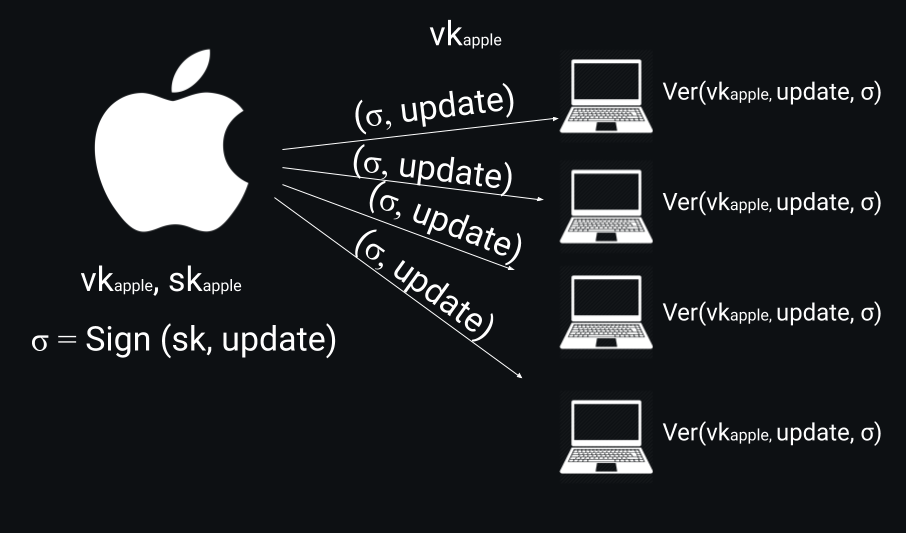
\includegraphics[width=0.9\textwidth]{Signature_software}
\end{figure}
\end{frame}

\begin{frame}{Схемы подписи на практике}
\Large
\begin{enumerate}
	\itemsep10pt
	\item {\color{Orange} RSA} \\
	-- основана на сложности задачи {\color{Orange} факторизации}\\
	-- быстрая процедура $\Ver$, медленные $\Sign, \KeyGen$; длинный ключи, подписи
	
	\item {\color{Orange} (EC)DSA= (Elliptic Curve) Digital Signature Algorithm} \\
	-- основана на сложности задачи  {\color{Orange} dlog}\\
	-- медленнее $\Ver$, быстрее $\Sign, \KeyGen$\\
	-- в ECDSA меньшего размера ключи и подписи
	\pause
	\item {\color{Orange} ГОСТ Р 34.10-2012 }  \\
	-- аналогичен ECDSA \\
	-- старый ГОСТ Р 34.10-94 аналогичен DSA
\end{enumerate}
\pause
\centering

Размеры ключей (в битах):\\[5pt]
\begin{tabular}{c | c| c}
	Security lvl. & ECDSA / ГОСТ'12 & RSA/DSA \\ \hline
	80 & 160 & 1024 \\
	128 & 256 & 4096 \\
	256 & 512 & 15360
\end{tabular}
\end{frame}

\begin{frame}
Часть II \\ [10pt]
\begin{LARGE}
	
	\color{Orange}
	\Huge  Арифметика в кольце целых чисел
	
\end{LARGE}
\end{frame}

\begin{frame}{Арифметика в кольце целых}
\Large 
{\color{Orange} Положим $N = p \cdot q$, где $p, q$ -- большие простые числа}

\begin{itemize}
	\item $\ZN = \left\{ 0, 1, \ldots, N-1 \right\}$ -- {\color{Orange} кольцо}
	\item Элементы $\ZN$ складываются и умножаются по модулю $N$. \\
	Пример: $N = 15$
	\begin{align*}
	11+6 \bmod N &= \rem(17, 15) = 2 \\
	6\cdot 7  \bmod N &= \rem(42, 15) = 12
	\end{align*}
	
	\item Не для всякого ненулевого $x \in \ZN$ существует обратимый! \\[3pt]
	Множество обратимых элементов: $\ZN^{\ast} =\{x \in \ZN \; | \;  \text{НОД}(x,N) = 1\}$.\\[5pt]
	
	Пример: $3, 6, 9, 5, 10, 12 \notin \ZN^{\ast}$. \\[3pt]
	$\ZN^{\ast} = \{1, 2, 4, 7, 8, 11, 13, 14\}$.
\end{itemize}

\end{frame}

\begin{frame}{Структура $\ZN^\ast$ }
\Large 
\begin{itemize}
\itemsep 10pt
\item  $\phi(N) = |\ZN^\ast|$ -- {\color{Orange}функция  Эйлера} \\[5pt]
--  $N$ -- простое, $\phi(N) = N-1$ \\[3pt]
--  $N = p_1^{e_1} \cdot p_n^{e_n}$, $\phi(N)=  N \cdot \prod_{i} \left(1 - \frac{1}{p_i}\right)$. \\[3pt]
-- для $N = p \cdot q$, {\color{Orange}$\phi(N) = (p-1)(q-1)$.} \\[3pt]
Пример: $|\ZN^{\ast}| = |\{1, 2, 4, 7, 8, 11, 13, 14\}| = 2 \cdot 4 = 8$.

\item {\color{Orange}Теорема Эйлера:} для всех $a \in \ZN^{\ast}$
\[
{\color{Orange}	\LARGE a^{\phi(n)} = 1 \bmod N }
\]
{\large Теорема Ферма: $a^{p-1} = 1 \bmod p$ для простого $p$.}
\end{itemize}
\end{frame}

\begin{frame}{Простые и трудные задачи в $\ZN$}
\Large 
\begin{center}
{\color{Orange}  $N = p \cdot q$},  $p, q$ -- по $\approx$ 1024/2048 бит каждое.\\
\end{center}
В $\ZN$ следующие операции  {\color{Orange} эффективные}  \\[5pt]
-- сложение, умножение, нахождение обратного (если существует, проверить несуществование)\\[3pt]
--  возведение в степерь $g^r \bmod N$ \\[14pt]
Сегодня  {\color{Orange} считаются трудными} задачи \\[5pt]
-- {\color{Orange} факторизация}: нахождение $p, q$  \\[3pt]
-- вычисление квадратного корня в $\ZN$ (эквивалентно факторизации) \\[3pt]
-- вычисление $e$-го корня в  $\ZN$ при $\gcd(e, \phi(N)) = 1$\\
%-- dlog (TODO)
\end{frame}


\begin{frame}
Часть III \\ [10pt]
\begin{LARGE}
	
	\color{Orange}
	\Huge  Подпись RSA
	
\end{LARGE}
\end{frame}



\begin{frame}{Генерация ключей в подписи RSA}
\Large
Возьмём $\ell>2$--целое и $e>2$ -- нечетное целое (на практике  $e=65537$) \\[8pt]
{\color{Orange} $\mathsf{RSAGen}(\ell, e):$}
\begin{enumerate}
	\itemsep5pt
	\item Сгенерировать $\ell$-битное целое $p$ т.ч.\ $\gcd(p-1, e)=1$
	\item Сгенерировать  $\ell$-битное цело $q \neq p$ т.ч.\ $\gcd(q-1, e)=1$
	\item $N= p \cdot q$, $\phi(N) = (p-1)(q-1)$
	\item $d = e^{-1} \bmod \phi(N)$
	\item Вывод: $\vk = (N, e), \sk=(N, d)$
\end{enumerate}
%\vspace{7pt}
\large
\pause
\begin{itemize}
	\item  $\exists$ ppt алгоритм генерации простых чисел ($\exists$  ppt алгоритмы теста на простоту)
	\item Шаг 4 корректен:  $d \in \ZN^\ast$, т.к. \[ \hspace{-20pt} \gcd(p-1, e) = \gcd(q-1, e) = 1 \implies \gcd((p-1)(q-1), e)=1.\]
	\item на $p,q$ должны удовлетворять  {\color{Orange} большому числу условий} 
\end{itemize}
\centering
\Large Не пытайтесь повторить $\mathsf{RSAGen}$ самостоятельно. 
\end{frame}

\begin{frame}{RSA Signature Generation and Verification}
\large
$\Hash: \{0,1\}^\ast \rightarrow \ZN^\ast$-- криптографическая хэш-функция
\vspace{10pt}
\begin{columns}[t]
\begin{column}{0.45\textwidth}
	
	{\color{Orange} I. $\mathsf{RSASign}(\sk=(N, d), m):$}
	\begin{enumerate}
		\itemsep5pt
		\item $y = \Hash(m) \in \ZN^\ast$
		\item $\sigma = y^d \bmod N$
	\end{enumerate}
	\vspace{10pt}
	\pause
	{\color{Orange} II. $\mathsf{RSAVerify}(\vk=(N, e), m, \sigma):$}
	\begin{enumerate}
		\itemsep5pt
		\item $y' = \sigma^e \bmod N$
		\item $\mathtt{return}(y'==\Hash(m))$ \\
	\end{enumerate}
\end{column}
\begin{column}{0.55\textwidth}
	\pause
	{\color{Orange} Корректность:}
	Для $N=pq$ и $e,d$ т.ч.\ $ed = 1 \bmod \phi(N)$ и для всех $x \in \Z$
	{\color{Orange} 
		\[
		x^{ed} = x \bmod N
		\] }
	\pause
	Док-во: для $k \in \Z$
	\begin{align*}
	&ed = 1 + k \phi(N) = 1+k(p-1)(q-1) \\  \pause
	& x^{p-1} = 1 \bmod p \quad \text{(Ferma't thm.)}\\ \pause
	& x^{ed} = x^{1+k(p-1)(q-1)} = \\
	& x \cdot (x^{p-1})^{q-1} = x \bmod p \\ \pause
	&\text{Аналог.}, x^{ed}  = x \bmod q \\ \pause
	& \implies  p, q \, |\, x^{ed} - x \\
	& \implies   x^{ed} = x \bmod p \cdot q
	\end{align*}
\end{column}
\end{columns}
\LARGE
%\vspace*{-40pt}
%{\color{Orange}  $(y^d)^e = y^{ed} = y \bmod N$ } \\[20pt]
\vspace{10pt}
\centering
\vfill
Без $\Hash$ схема тривиально взламывается!
\end{frame}

\begin{frame}{Безопасность подписи RSA}
\Large

{\color{Orange}  RSA предположение сложности:}
Не существует ppt алгоритма, который, получив на вход $(N, m, m^e)$ для случайного $m \in \ZN^\ast$, выдаёт $m$.\\[10pt]

{\centering Факторизация $N \implies $ вычисление $e$-го корня. \\[5pt] Обратная редукция не доказана! }  \\[15pt]

Самый быстрый сегодня алгоритм факторизации -- General Number Field sievie -- со сложностью
\[
\sim e^{(\lg N)^{1/3}}
\]


{\color{Orange}  Теорема:} Схема подписи ($\mathsf{RSAGen},$ $\mathsf{RSASign},$ $\mathsf{RSAVerify}$) безопасна в \\ модели {\color{Orange} UF-CMA}, если {\color{Orange}  предположение RSA корректно} и $\Hash$ является \\ {\color{Orange}  случайным оракулом.} \\[10pt]

\end{frame}

\begin{frame}{Стандарты}
\Large 
Вариант RSA подписи станартизованы под именем PKCS (Public Key Cryptography Standards)   \\
\url{https://en.wikipedia.org/wiki/PKCS} \\[10pt]

Версия 2.2 (крайняя)  PKCS \#1 включает \\[10pt]
\begin{itemize}
\itemsep10pt
\item RSASSA-PSS \\
SSA = Signature Scheme with Appendix \\[5pt]
PSS =  Probabilistic Signature Scheme
\item  RSASSA-PKCS1-v1\_5 (существуеют атаки)
\end{itemize}

\end{frame}

\begin{frame}
Часть IV \\ [10pt]
\begin{LARGE}
	
	\color{Orange}
	\Huge  Слепая подпись. Сертификаты
	
\end{LARGE}
\end{frame}


\begin{frame}{ Слепая подпись RSA}

\Large
{\color{Orange} Сценарий:} {\color{Orange} A }  необходима подпись банка ({\color{Orange} Б}) на осуществлении транзакции. При этом {\color{Orange} Б } не должен знать о том, что именно он подписывает. {\color{Orange} Б } осуществляет {\color{Orange} слепую подпись.} \\[5pt]

$\Hash: \{0,1\}^\ast \rightarrow \Z_p^\ast$ -- криптографическая хэш-функция \\
$ m $ -- транзакция

\begin{center}
	\begin{tabular}{c c c}
		{\color{Orange} A } & & {\color{Orange} Б }\\ [5pt]
		& &  $\sk = (N, d), \vk= (N, e)\leftarrow \mathtt{RSA.KeyGen()}$\\
		$r \xleftarrow{\$} \Z_N$ & &  \\
		$m' = \Hash(m) \cdot r^e$  & $\xrightarrow{ \Huge \; m' \;}$&  $\sigma' = (m')^d$ \\
		$\sigma = \sigma' / r $& $\xleftarrow{ \Huge \; \sigma' \;}$&  \\
	\end{tabular}
	
\end{center}

\begin{itemize}
	\item {\color{Orange} A } получает корректную подпись для $m'$ \\[25pt]
	\item Значение $r^e$ маскирует исходное сообщение ({\color{Orange} Б} не знает ничего о $m$)
\end{itemize}

\end{frame}



\begin{frame}{Слепая подпись }

\Large

\begin{itemize}
\itemsep10pt
\item Слепая подпись безопасна, если ppt атакующий, зная $\vk$ и $Q$ слепых подписей, не может сгенерировать $Q+1$ пару  $(m, \sigma)$
\item Безопасность слепой подписи RSA основана на задача 1MRSA: \\
\begin{itemize}
	\itemsep5pt
	\large 
	\item {\color{Orange} A} получает значения $w = \hat{v}^{1/e}$ от Челленджера для $\hat{v}$ по своему выбору
	\item Задача {\color{Orange} A}: вычислить $v^{1/e}$ для какого-либо одного $v \neq \hat{v}$, выбранного Челленджером
\end{itemize}	

\item Слепая подпись может быть построена на основе подписи Шнорра
\item Используются в протоколах Anonymous Credentials, E-cash. 
\end{itemize}


\end{frame}

\begin{frame}{Применение криптографических подписей}
\Large
Подписи на практике
\begin{enumerate}
\itemsep 10pt
\item RSA \\
длинные ключи и подписи; быстрая верификация
\item ECDSA, ГОСТ\\
короткие ключи и подписи; верификация медленнее
\end{enumerate}
\vspace{10pt}
RSA хороша для {\color{Orange} Сертификатов}, ECDSA/ГОСТ -- для имейлов. \\[10pt]


\end{frame}

\begin{frame}{Сертификаты}
\Large 
Задача сертификата:  связать публичный ключ с человеком/машиной.
\begin{center}
\begin{tabular}{l c c c l}
& \Large Алиса & &\Large Сертификационный центр (CA)&  \\ 
&  $\pk_{\texttt{A}}$  & & $\vk_{\texttt{CA}}$, $\sk_{\texttt{CA}}$ & \\
& \multirow{5}{*}{
\includegraphics[scale=0.15]{Alice}} & & &  \\  \pause
& & $\xrightarrow[\texttt{id, email, } \pk_{\texttt{A}}]{\text {Certificate Signing Request}}$ & & \\  \pause
& & & \Large Сертификация id Алисы: & \\
& & & Создание $\texttt{cert}$& \\
& & & Подпись $\texttt{cert}$& \\
& & $\xleftarrow{\LARGE \texttt{cert}, \; \sigma = \Sign(\sk_{\texttt{CA}}, \texttt{cert})}$ & & \\  
\end{tabular}
\end{center}

\vspace{15pt}
\Large
Для осуществления аутентифицированного канала с Алисой \\
верифицируется $\texttt{cert}$:
$\Ver(\vk_{\texttt{CA}} \texttt{cert},\sigma )$. \\[5pt]

Если $\Ver(\vk_{\texttt{CA}} \texttt{cert},\sigma ) = \mathsf{accept}$, то $\pk_{\texttt{A}}$ используется для \\ коммуникации с Алисой.\\[8pt]

Пример: сертификат X.509 certificate
\end{frame}

\begin{frame}{Цепочки сертификатов}
\Large
\begin{center}

\begin{align*}
&{\LARGE \text{Корневой CA } \hspace{70pt} \xrightarrow{\hspace{2em}} \quad \quad \text{Промежуточный CA}} \\
&\text{сертифицирует промежуточные CA}  \hspace{37pt} \text{сертифицирует клиентов} 
\end{align*}
\end{center}
\vspace{15pt}
Сегодня мы имеем тысячи промежуточный CAs \\[10pt]
Для противостояния CAs: {\color{Orange} certificate pinning:} \\[7pt]
\begin{enumerate}
\item Каждый браузер (клиент) поддерживает базу данных (pinning database): \\
($\texttt{domain}$, $\texttt{hash}_0$, $\texttt{hash}_1, \ldots$ )
\item Данные для БД предоставляет домен
\item Когда браузер стучится в домен, домен высылает ему цепочку\\ своих сертификатов $\texttt{cert}_0, 
\texttt{cert}_1, \ldots$
\item Браузер вычисляет $\Hash(\texttt{cert}_i)$ и верифицирует $\texttt{hash}_i$. 
\end{enumerate}

\end{frame}

\begin{frame}{Пример цепочки сертификатов }
\begin{figure}
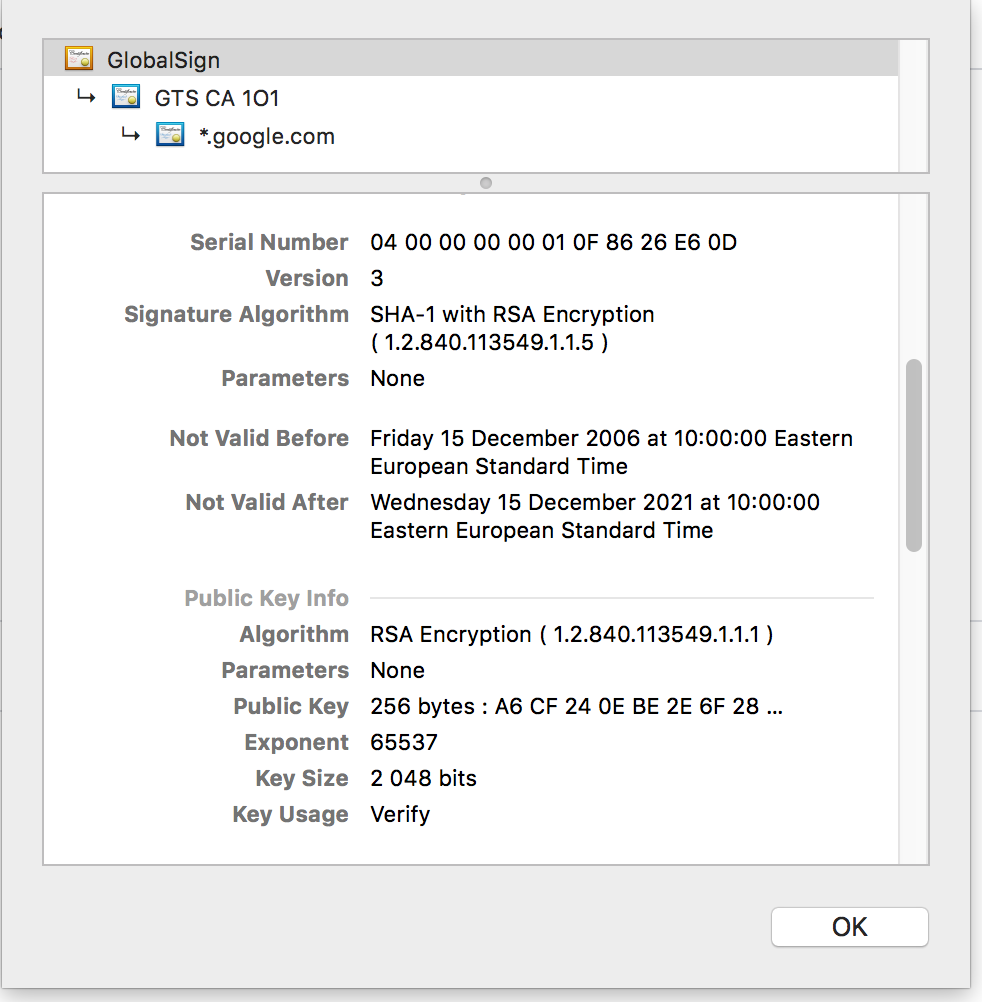
\includegraphics[scale=0.45]{cert1}
\end{figure}


\end{frame}


\end{document}
